\let\negmedspace\undefined
\let\negthickspace\undefined
\documentclass[journal]{IEEEtran}
\usepackage[a5paper, margin=10mm, onecolumn]{geometry}
%\usepackage{lmodern} % Ensure lmodern is loaded for pdflatex
\usepackage{tfrupee} % Include tfrupee package

\setlength{\headheight}{1cm} % Set the height of the header box
\setlength{\headsep}{0mm}     % Set the distance between the header box and the top of the text

\usepackage{gvv-book}
\usepackage{gvv}
\usepackage{cite}
\usepackage{amsmath,amssymb,amsfonts,amsthm}
\usepackage{algorithmic}
\usepackage{graphicx}
\usepackage{textcomp}
\usepackage{xcolor}
\usepackage{txfonts}
\usepackage{listings}
\usepackage{enumitem}
\usepackage{mathtools}
\usepackage{gensymb}
\usepackage{comment}
\usepackage[breaklinks=true]{hyperref}
\usepackage{tkz-euclide} 
\usepackage{listings}
% \usepackage{gvv}                                        
\def\inputGnumericTable{}                                 
\usepackage[latin1]{inputenc}                                
\usepackage{color}                                            
\usepackage{array}                                            
\usepackage{longtable}                                       
\usepackage{calc}                                             
\usepackage{multirow}                                         
\usepackage{hhline}                                           
\usepackage{ifthen}                                           
\usepackage{lscape}
\begin{document}

\bibliographystyle{IEEEtran}
\vspace{3cm}
\title{1.1.6-21}
\author{EE24BTECH11028 - Jadhav Rajesh}
% \maketitle
% \newpage
% \bigskip
{\let\newpage\relax\maketitle}

\renewcommand{\thefigure}{\theenumi}
\renewcommand{\thetable}{\theenumi}
\setlength{\intextsep}{10pt} % Space between text and floats


\numberwithin{equation}{enumi}
\numberwithin{figure}{enumi}
\renewcommand{\thetable}{\theenumi}
 \textbf{Question:} Show that points A$\vec(a,b+c)$, B$\vec(b,c+a)$, C$\vec(c,a+b)$ are collinear.\\
 \solution let the coordinates of the points be \\
              A$\vec(a,b+c)$\\
              B$\vec(b,c+a)$\\
              C$\vec(c,a+b)$\\
        we can set up the matrix as follows\\
    \begin{align}
          \triangle = \myvec{
                              a & b+c & 1\\
                              b & c+a & 1\\
                              c & a+b & 1}
    \end{align} 
    using row operation\\
    \begin{align}
                   R_{2}\rightarrow{R_{2}-R_{1}}\\
                   R_{3}\rightarrow{R_{3}-R{1}}
    \end{align}
    \begin{align}
                  \myvec{
                         a & b+c & 1\\
                         b & \vec(c+b)-\vec(b+c) & 1-1\\
                         c & \vec(a+b)-\vec(b+c) & 1-1}
    \end{align}
    \begin{align}
                    \myvec{
                            a & b+c & 1\\
                            b-a & a-b & 0\\
                            c-a & a-c & 0}
    \end{align}
                expanding alone the colume third\\
    \begin{align}
                   \myvec{
                           b-a & a-b\\
                           c-a & a-c}
    \end{align}
                  by using coulme operation
    \begin{align}
                C_{1}\rightarrow{C_{1}+C_{2}}
    \end{align}
    \begin{align}
                    \myvec{
                           0 & a-b\\
                           0 & a-c}
    \end{align}
               the above process is known as coulme reduced matrix is defined as the rank.\\
               Define the coordinates of point A, B,, and C
    \begin{align}
             a,b,c = 1,2,3
    \end{align}

     \begin{figure}[h!]
	   \centering
	  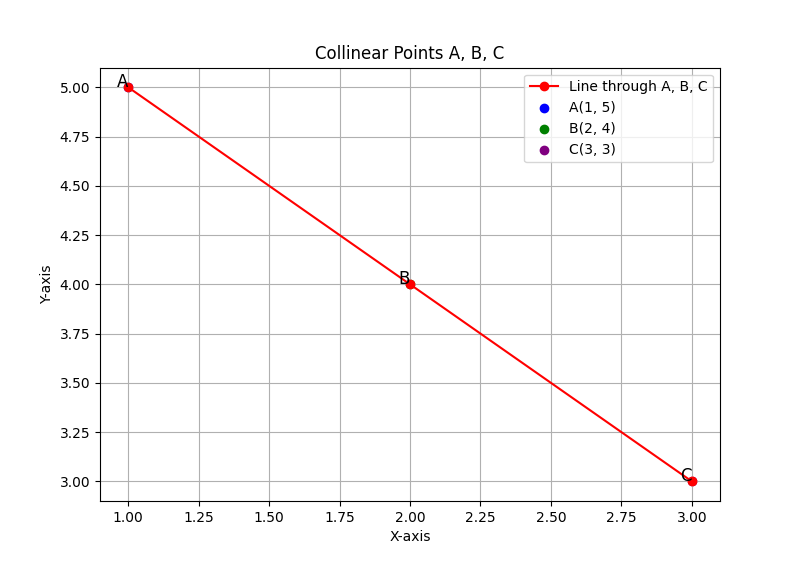
\includegraphics[width=0.5\linewidth]{Figure_1.jpg}
	\caption{ $\vec{A}\vec{B}\vec{C}$Collinear points}


	  \label{stemplot}
    \end{figure}
              
    
                  
 
\end{document}


